
\noindent\begin{minipage}{\textwidth}
    \begin{table}[H]
        \centering
        \caption{Hiperparâmetros e Resultados do Melhor Modelo - convnext\_v1\_AB\_opt\_aug}
        \vspace{0.2cm}
        \resizebox{\textwidth}{!}{%
            \begin{tabular}{ll | lrrr}
                \hline
                \multicolumn{2}{c|}{\textbf{Hiperparâmetros}} & \multicolumn{4}{c}{\textbf{Métricas por Classe}} \\ \hline
                \textbf{Parâmetro} & \textbf{Valor} & \textbf{Classe} & \textbf{Precisão} & \textbf{Recall} & \textbf{F1-Score} \\ \hline
    Agendador (\$T\_0\$) & 12 & 31.2 & 0,8112 & 0,5133 & 0,6287 \\ 
Agendador de LR & CosineAnnealingWarmRestarts & 31.3 & 0,4727 & 0,7277 & 0,5731 \\ 
Architecture & convnext\_tiny & 31.4 & 0,4654 & 0,7048 & 0,5606 \\ 
Aug (Brilho / Contraste) & 0,20 / 0,19 & 32.3 & 0,6522 & 0,6122 & 0,6316 \\ 
Aug (Prob. Espelhamento) & 0,22 & 32.4 & 0,7250 & 0,5000 & 0,5918 \\ 
Aug (Rotação) & 13\$\textasciicircum{}\textbackslash{}circ\$ & 33.3 & 0,7852 & 0,6062 & 0,6842 \\ 
Augmentation (Método) & Basic & 41.4 & 0,8095 & 0,3864 & 0,5231 \\ 
Batch Size & 32 & 41.5 & 0,8000 & 0,7179 & 0,7568 \\ 
Decaimento de Peso (WD) & 0,0243 & 42.4 & 0,9167 & 0,4853 & 0,6346 \\ 
Dropout & 0,2537 & 44.4 & 0,8214 & 0,7931 & 0,8070 \\ 
\cline{3-6} 
Função de Perda & CrossEntropyLoss & \textbf{Média (Macro)} & 0,6511 & 0,6864 & 0,6638 \\ 
Hidden Units & 512 & \textbf{MCC} & \multicolumn{3}{c}{0,6053} \\ 
Label Smoothing & 0,1507 &  & & &  \\ 
Otimizador & AdamW &  & & &  \\ 
Taxa de Aprendizado (LR) & 2,85e-04 &  & & &  \\ 
Unfreeze Layers & 5 &  & & &  \\ 
            \hline
            \end{tabular}%
        }
    \end{table}

    \begin{figure}[H]
        \centering
        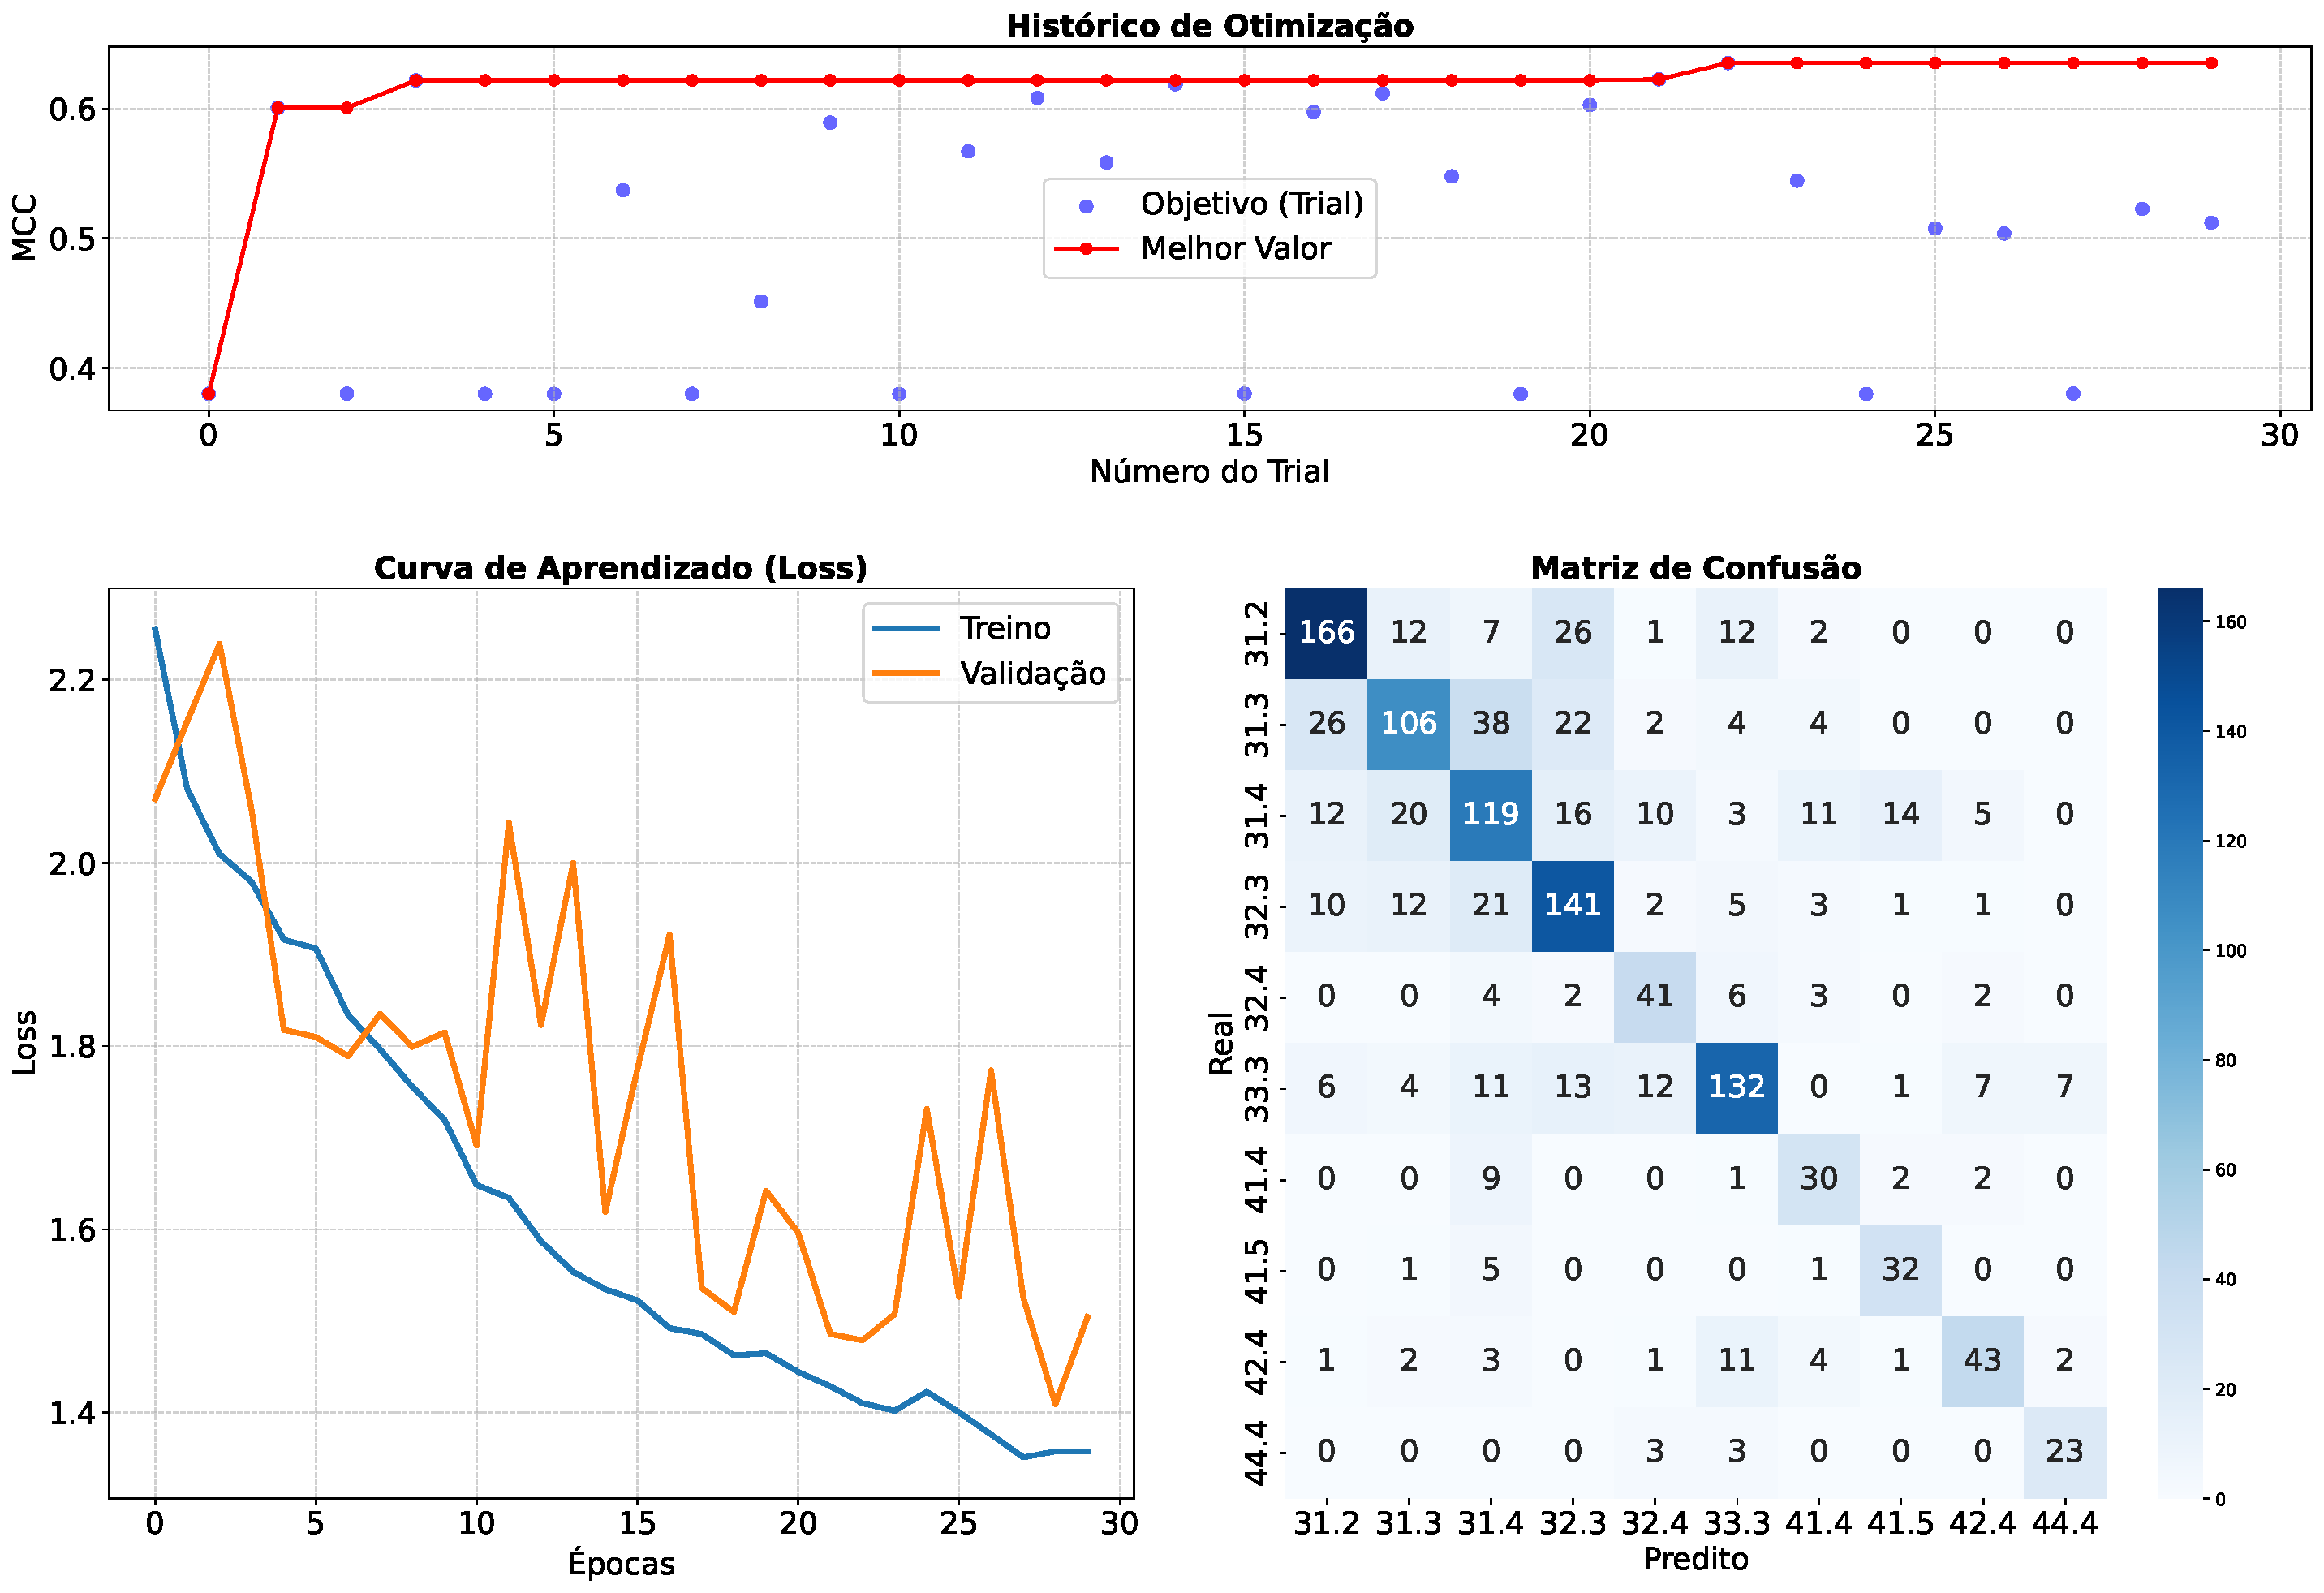
\includegraphics[width=0.85\textwidth]{tex/appendix/experiments/convnext_v1_AB_opt_aug/dashboard_consolidado.pdf}
        \caption{Histórico de Otimização, Curvas de Aprendizado e Matriz de Confusão - convnext\_v1\_AB\_opt\_aug}
    \end{figure}
\end{minipage}
\clearpage
